\PassOptionsToPackage{svgnames}{xcolor}
\documentclass{report}
% \usepackage[utf8]{inputenc}
\usepackage[left=2cm,right=2cm,top=2cm,bottom=2cm]{geometry}
\usepackage{hyperref}
\usepackage{amsmath}
\usepackage{graphicx}
\usepackage{import}
\usepackage{float} % for H option in figure
\usepackage{enumitem}
\usepackage{pifont}
\hypersetup{
    colorlinks=true,
    linkcolor=blue,
    urlcolor=blue,
    citecolor=blue
}
\usepackage{tcolorbox}

\definecolor{MainColor}{RGB}{0,82,82} % dark teal


% -----------------------------------------------------------------------------
% Font
% see https://tug.org/FontCatalogue/firasans/
% 'sfdefault' activates Fira Sans as the default text font
% 'lining' increases numbers height
\usepackage[sfdefault,lining,light]{FiraSans}
\usepackage[T1]{fontenc}
% \renewcommand*\oldstylenums[1]{{\firaoldstyle #1}} ???
\usepackage{FiraMono} % only for monospaced texttt
% \usepackage[ttscale=.875]{libertine}
% \usepackage{time}
%
% fix default extreme Fira bold for each section, subsection...
\usepackage{titlesec} % \titleformat
\titleformat{\section}
{\normalfont\fontseries{sb}\Large\color{MainColor}}
{Étape~\thesection.}{1em}{}
%
\titleformat{\subsection}
{\normalfont\fontseries{m}\large\color{MainColor}}
{\thesubsection}{0.5em}{}
%
\titleformat{\subsubsection}
{\normalfont\fontseries{m}\normalsize\color{MainColor}}
{\thesubsubsection}{0.4em}{}
%
\titleformat{\paragraph}[runin]
{\normalfont\fontseries{m}\normalsize\color{MainColor}}
{\theparagraph}{}{}
%
\titleformat{\subparagraph}[runin]
{\normalfont\fontseries{m}\normalsize\color{MainColor}}
{\thesubparagraph}{}{}
%

\counterwithout{section}{chapter}
\setcounter{section}{-1}

\newcommand{\step}{\item[\textcolor{MainColor}{\ding{237}}]}
\newcommand{\code}[1]{\texttt{"#1"}}
\newcommand{\cmd}[1]{\texttt{#1}}

\begin{document}

% ----------------------------------------------------------------
\begin{titlepage}
\begin{center}

    \vspace*{2cm}

    {\huge\bfseries\textcolor{MainColor}{Journée d'Immersion - Atelier Robotique}}

    \vspace{2cm}

    {\Large\textcolor{MainColor}{EPITA Toulouse}}

    \vspace{2cm}

    
\includegraphics[width=0.75\textwidth]{img/epita.png}

    \vspace{4cm}

    {\large\textcolor{MainColor}{20 janvier 2024}}

\end{center}
\end{titlepage}
% ----------------------------------------------------------------



%%%%%%%%%%%%%%%%%%%%%%%%%%%%%%%%%%%%%%%%%%%%%%%%%
\section{Mise en place du simulateur}
%%%%%%%%%%%%%%%%%%%%%%%%%%%%%%%%%%%%%%%%%%%%%%%%%

\begin{itemize}
    \step Ouvrir un terminal en cliquant sur l'icône \raisebox{-1mm}{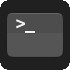
\includegraphics[width=6mm]{img/logo_terminal.jpg}} dans la barre de lancement à gauche.
    \step Dans le terminal, entrer la commande \texttt{"robotSimulateur"} et appuyez sur la touche entrée.
\end{itemize}

\begin{center}
    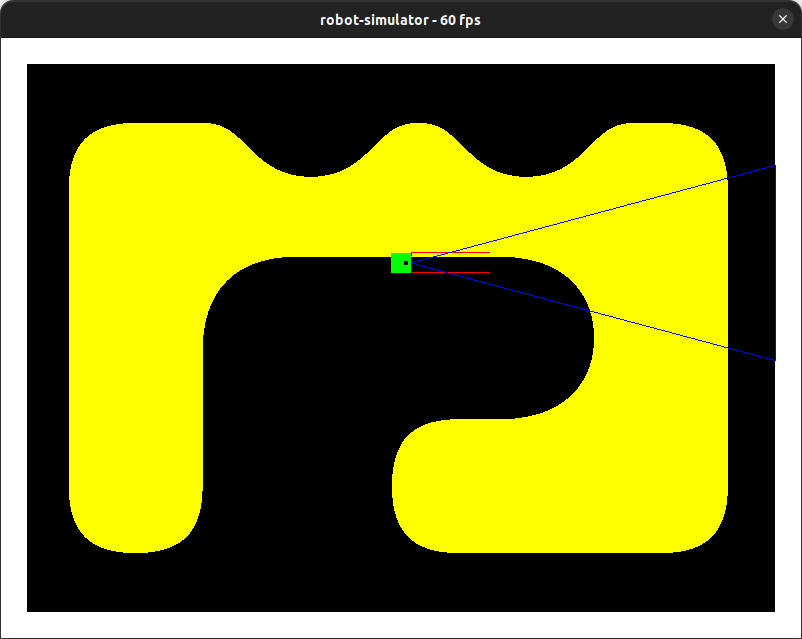
\includegraphics[width=0.7\linewidth]{img/simu.png}
\end{center}

\subsection{Description}

Le simulator affiche une vue de dessus du robot et de son environnement avec les éléments suivants :
\begin{itemize}
    \item[-] Carré vert : robot
    \item[-] Ligne rouge : télémètre infrarouge
    \item[-] Cône bleu : télémètre ultrason
    \item[-] Pixels blancs : mur
    \item[-] Pixels noir et jaune : couleur du sol
\end{itemize}

\subsection{Touches de contrôle du simulateur}

Le robot peut être guidé manuellement grâce aux touches suivantes :
\begin{itemize}
    \item[-] Flèches directionnelles : guider le robot
    \item[-] Touche espace : réinitialiser la position du robot
\end{itemize}

\begin{itemize}
    \step Tester le simulateur manuellement en guidant le robot à travers l'environnement.
\end{itemize}




%%%%%%%%%%%%%%%%%%%%%%%%%%%%%%%%%%%%%%%%%%%%%%%%%
\section{Lancement de l'environnement de développement}
%%%%%%%%%%%%%%%%%%%%%%%%%%%%%%%%%%%%%%%%%%%%%%%%%

\subsection{Lancement}

\begin{itemize}
\step Lancer VS~Code en cliquant sur l'icône \raisebox{-1mm}{
\includegraphics[width=6mm]{img/logo_vscode.jpg}} dans la barre de lancement à gauche.
\step Cliquer sur le menu \texttt{"File"}, puis sur l'option \texttt{"Open Folder"}, sélectionner le dossier \texttt{"workspace"}, puis le dossier \texttt{"robot-command-py"}, enfin cliquer sur \texttt{"Open"}.
\step Ouvrir le fichier \texttt{"main.py"} en cliquant dessus sur le panneau de gauche de VS~Code.
\step Chercher la ligne contenant \texttt{"def step1\_move3s(robot:~Robot):"}
    \begin{itemize}
    \item[-] \texttt{"robot.setMotorsSpeed(0.2, 0.2)"} signifie "avancer tout droit"
    \item[-] \texttt{"time.sleep(3.0)"} signifie "attendre pendant 3 secondes"
    \item[-] \texttt{"robot.setMotorsSpeed(0.0, 0.0)"} signifie "stopper les 2 roues du robot"
    \end{itemize}
\step Lancer le programme en cliquant sur le triangle blanc \raisebox{-1mm}{
\includegraphics[width=6mm]{img/logo_play.jpg}} en haut à droite, puis observer le robot sur le simulateur.
\end{itemize}

\subsection{Description du code}

Dans le code Python que nous allons utiliser, il y a une variable \code{robot} sur laquelle nous allons utiliser la
fonction \code{robot.setMotorsSpeed(rightValue, leftValue)} qui permet de modifier la vitesse des
moteurs des roues du robot.
Il y a $2$ paramètres correspondant aux $2$ roues du robot.
Pour chacune des roues, les valeurs de vitesse sont comprises entre $-1.0$ et $+1.0$ :
\begin{itemize}
\item[$+1.0$] en avant à vitesse maximale
\item[$\phantom{+}0.0$] arrêt du moteur
\item[$-1.0$] en arrière à vitesse maximale
\end{itemize}




%%%%%%%%%%%%%%%%%%%%%%%%%%%%%%%%%%%%%%%%%%%%%%%%%
\section{1\textsuperscript{er} programme : tourner}
%%%%%%%%%%%%%%%%%%%%%%%%%%%%%%%%%%%%%%%%%%%%%%%%%

\begin{itemize}
\step Dans le fichier \texttt{"main.py"}
\step Remplacer \code{TODO step2} par le pseudo-code suivant (en vous inspirant de la fonction \code{step1\_move3s})
\begin{itemize}
    \item[-] faire tourner le robot sur lui-même
    \item[-] attendre 3 secondes
    \item[-] arrêter le robot
\end{itemize}
\step A la fin du fichier (dans le \texttt{"main"}) :
\begin{itemize}
    \step commenter la ligne \code{step1\_move3s(robot)} (rajouter \code{\#} devant la ligne)
    \step décommenter la ligne \code{step2\_turn3s(robot)} (enlever \code{\#} devant la ligne)
\end{itemize}
\step Lancer le programme en cliquant sur le triangle blanc \raisebox{-1mm}{
\includegraphics[width=6mm]{img/logo_play.jpg}} en haut à droite
\end{itemize}

\paragraph{Remarque 1}
vérifier que lorsque le programme est lancé, le terminal de VS~Code affiche bien les lignes
\begin{itemize}
\item[-] \texttt{"Création du robot"}
\item[-] \texttt{"Lancement du programme"}
\item[-] \texttt{"Fin du programme"}
\item[-] \texttt{"\textasciitilde/workspace/robot-command-py\$"}
\end{itemize}
Si ce n'est pas le cas, le programme est bloqué, faire alors un \texttt{"ctrl-c"} dans la console pour le débloquer.

\paragraph{Remarque 2}
Essayer de faire varier le centre de rotation du robot en modifiant les vitesses des roues droite et gauche du robot.






%%%%%%%%%%%%%%%%%%%%%%%%%%%%%%%%%%%%%%%%%%%%%%%%%
\section{1\textsuperscript{er} évènement : se déplacer jusqu'au mur}
%%%%%%%%%%%%%%%%%%%%%%%%%%%%%%%%%%%%%%%%%%%%%%%%%

\begin{itemize}
\step Remplacer \texttt{"TODO step3"} par le pseudo-code suivant
\begin{itemize}
    \item[-] avancer en ligne droite
    \item[-] attendre d'être en collision avec le mur en utilisant \texttt{"robot.waitChanged(robot.EventType.SWITCH)"}
    \item[-] arrêter le robot
\end{itemize}
\end{itemize}

\paragraph{Remarque}
Penser à commenter et décommenter les fonctions à la fin du programme comme dans l'étape~2.

%%%%%%%%%%%%%%%%%%%%%%%%%%%%%%%%%%%%%%%%%%%%%%%%%
\section{1\textsuperscript{ère} boucle : figure géométrique}
%%%%%%%%%%%%%%%%%%%%%%%%%%%%%%%%%%%%%%%%%%%%%%%%%

\begin{itemize}
\step Remplacer \texttt{"TODO step4"} par le code suivant
    \begin{itemize}
        \item[] \texttt{while True:}
        \item[] \hspace{5mm} \texttt{robot.setMotorsSpeed(0.2, 0.2)}
        \item[] \hspace{5mm} \texttt{time.sleep(2.0)}
        \item[] \hspace{5mm} \texttt{robot.setMotorsSpeed(-0.1, 0.1)}
        \item[] \hspace{5mm} \texttt{time.sleep(0.5)}
    \end{itemize}
\end{itemize}

\paragraph{Remarque}
Respecter bien les indentations du code Python.

%%%%%%%%%%%%%%%%%%%%%%%%%%%%%%%%%%%%%%%%%%%%%%%%%
\section{1\textsuperscript{er} algorithme : explorer la pièce}
%%%%%%%%%%%%%%%%%%%%%%%%%%%%%%%%%%%%%%%%%%%%%%%%%

\begin{itemize}
\step Remplacer \texttt{"TODO step5"} par le pseudo-code suivant
\begin{itemize}
    \item[-] boucle infinie :
    \begin{itemize}
        \item[-] avancer en ligne droite
        \item[-] attendre d'être en collision avec le mur
        \item[-] reculer un peu
        \item[-] tourner un peu
    \end{itemize}
\end{itemize}
\end{itemize}

%%%%%%%%%%%%%%%%%%%%%%%%%%%%%%%%%%%%%%%%%%%%%%%%%
\section{Algorithme avancé : suivi de ligne}
%%%%%%%%%%%%%%%%%%%%%%%%%%%%%%%%%%%%%%%%%%%%%%%%%

\begin{itemize}
\step Remplacer \texttt{"TODO step6"} par un algorithme qui permet de faire un suivi du bord de la forme jaune
\step Vous aurez besoin de
    \begin{itemize}
    \item[-] boucle infinie :
    \begin{itemize}
    \item[-] attendre l'évènement de changement de couleur du sol :
    \item[]  \texttt{"robot.waitChanged(robot.EventType.LINE\_TRACK\_IS\_DETECTED)"}
    \item[-] lire la couleur du sol : \texttt{"robot.getLineTracksIsDetected(0)"} qui renvoi \texttt{"True"} ou \texttt{"False"} selon si la couleur est jaune ou noire
    \item[-] exécuter une action en fonction d'une condition
        \begin{itemize}
            \item[] \texttt{if} $<$\textit{condition}$>$ \texttt{:}
            \item[] \hspace{5mm} $<$\textit{action-vrai}$>$
            \item[] \texttt{else:}
            \item[] \hspace{5mm} $<$\textit{action-faux}$>$
        \end{itemize}
    \end{itemize}
    \end{itemize}
\end{itemize}

\end{document}